\section{การทำงานร่วมกันระหว่าง HAPS และ Terrestrial Networks}

เทคนิค Interference สามารถใช้เพื่อประสานการทำงานระหว่าง HAPS และ TN ได้
นั่นก็เพื่อ Utilize ทรัพยากรทั้งบน HAPS และ TN ให้มากขึ้น
โดยรูปแบบของการประสานการทำงานนั้นเป็นไปตามรูปที่ \ref{fig:03-different-cases}

\begin{figure}[h]
\caption[Different interference cases]{Different cases based on the traffic distribution and the deployment of integrated system} \label{fig:03-different-cases}
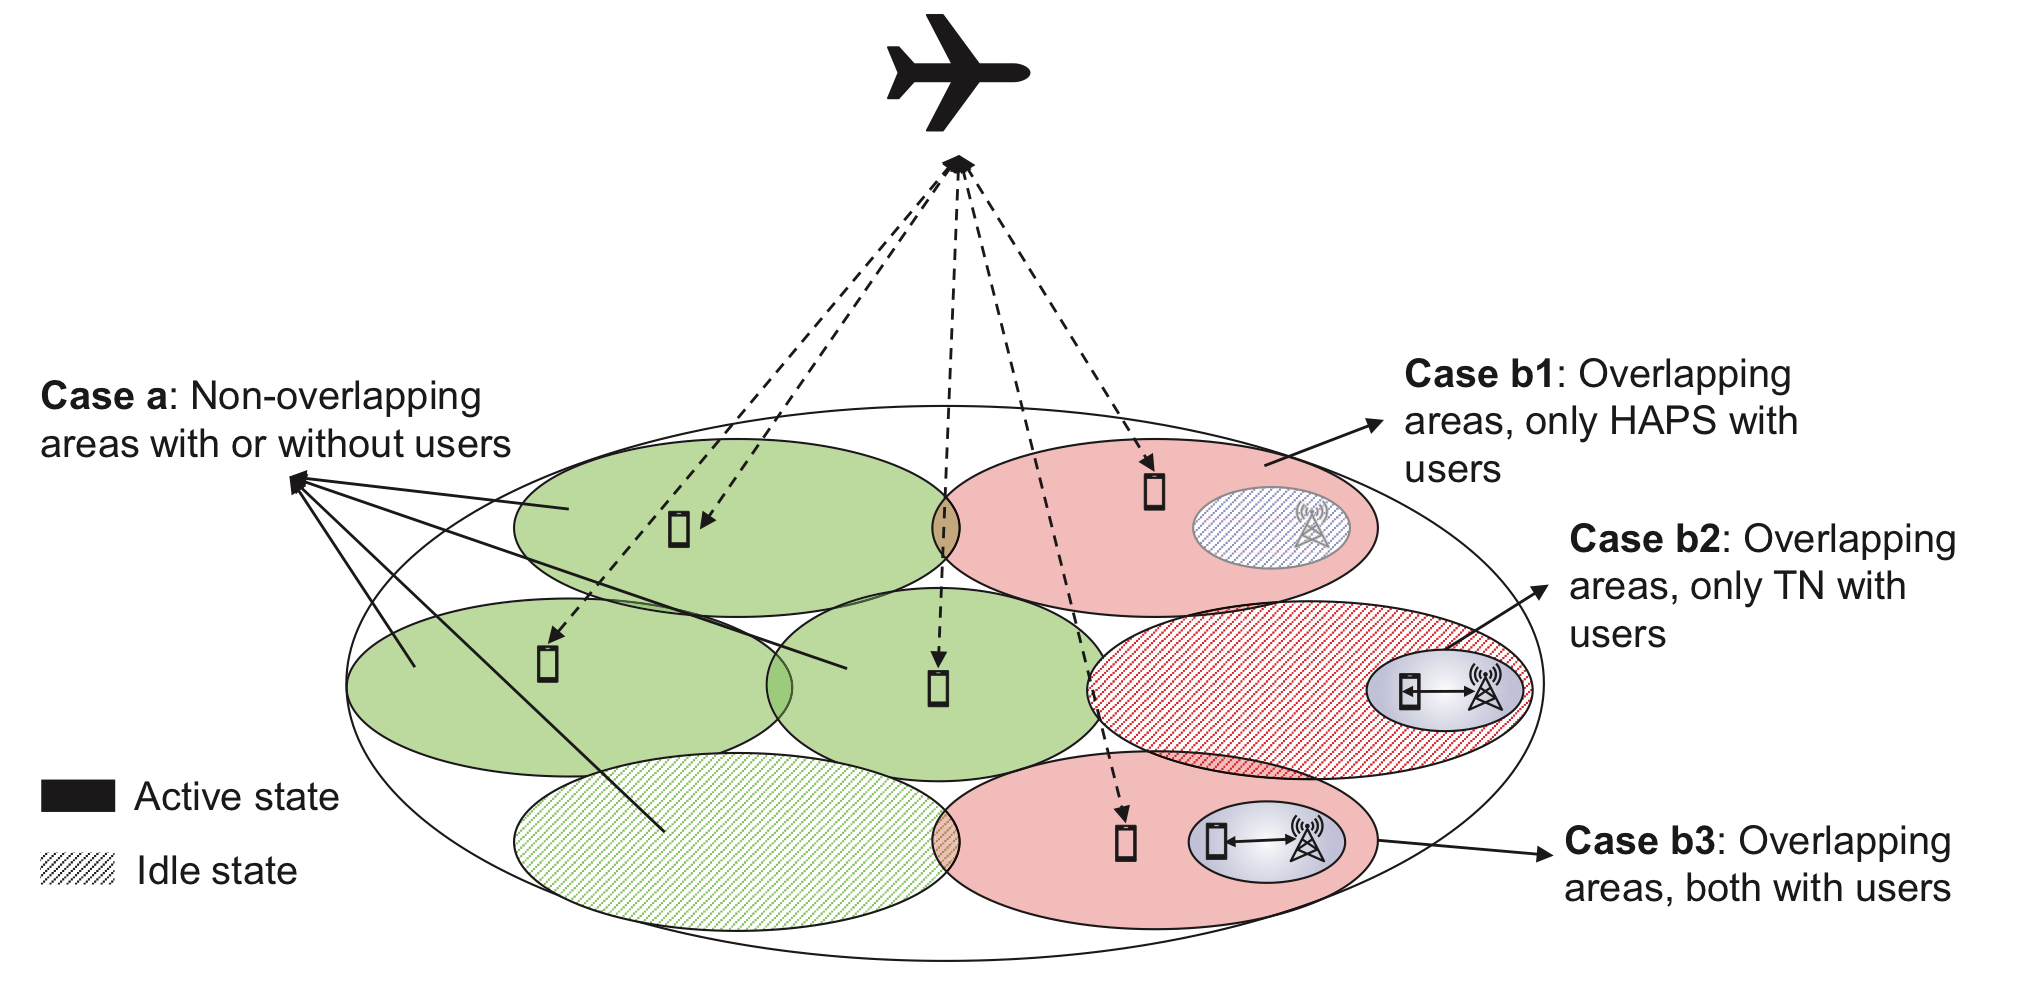
\includegraphics[width=0.7\textwidth]{03_different-cases.jpeg}
\end{figure}

\subsection{Non-overlapping Areas}

\subsection{Overlapping Areas Between HAPS and Terrestrial Coverage}
